

\documentclass{beamer}

\usepackage{simlab}
%minted: for python code. 
\usepackage{minted}

% Replace short paper title (inside square brackets) by our lab name
\title[Artifical Neural Networks]
{Artificial Neural Networks}
\subtitle{}
\date{\today}

%\subtitle{Include Only If Paper Has a Subtitle}

% Give the names in the same order as they appear in the paper.
% Use the \inst{?} command only if the authors have different affiliation.
% Names inside square brackets will appear at the bottom of each slide.
\author[Mitchell Corbett/Matthew Galbraith]{Mitchell Corbett and Matthew Galbraith}



% Uncomment this if you want the table of contents to pop up at the beginning of
% each subsection:
%\AtBeginSubsection[] {
%  \begin{frame}<beamer>
%  \frametitle{Outline}
%  \tableofcontents[currentsection,currentsubsection]
%  \end{frame}
%}

\begin{document} 
 
% If you wish to uncover everything in a step-wise fashion, uncomment the
% following command: 
%\beamerdefaultoverlayspecification{<+->}
\maketitle


% Comment the following lines if you wish to hide frame number
\expandafter\def\expandafter\insertshorttitle\expandafter{%
  \insertshorttitle\hfill%
  \insertframenumber\,/\,\inserttotalframenumber}

\begin{frame}
  \frametitle{Outline}
  \tableofcontents[pausesections]
  % You might wish to add the option [pausesubsections] as well.
\end{frame}

%---------------------------------------------------------------------- SECTION
\section{Introduction to ANN}
\begin{frame}
\frametitle{What is a Neural Network?}

\begin{itemize}
	\item What is a Neural Network?
    
\end{itemize}
\end{frame}
\subsection{Biological Inspirations}
\begin{frame}
\frametitle{Biological Inspirations}
\begin{itemize}
	\item In Biology, the Neuron is a fundamental unit of the Central Nervous System. It contains 3 parts. The Cell Body, Dendrites, and an Axon.
	\begin{itemize}
		\item The Cell Body contains the essential parts of the cell
		\item Dendrites are short fibers that receive signals.
		\item The Axon is a long projecting branch which sends signals. It can branch in to many other cells.
\end{itemize}
\end{itemize}
\end{frame}
\begin{frame}
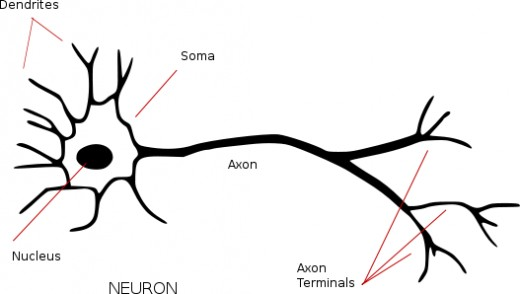
\includegraphics[width = 350px]{neuron.jpg}
\end{frame}

\subsection{Different Definitions}
\begin{frame}
\frametitle{DARPA NN Study}
\begin{itemize}
	\item "...a Neural Network is a system composed of many simple processing elements operating in parallel whose function is determined by network structure, connection strength and the processing performed at computing elements or nodes"
\end{itemize}
\end{frame}

\begin{frame}
\frametitle{Haykin (1994)}
\begin{itemize}
\item A neural network is a massively parallel distributed processor that has a natural propensity for storing experiential knowledge and making it available for use. It resembles the brain in two respects: 
  Knowledge is acquired by the network through a learning process. 
  Interneuron connection strengths known as synaptic weights are used to store the knowledge.
\end{itemize}
\end{frame}
\subsection{Applications}
\begin{frame}
\begin{itemize}
\item Classification
\end{itemize}
\end{frame}

\begin{frame}
\begin{itemize}
\item With that, let's dive in!
\end{itemize}
\end{frame}

\section{Feed-Forward Neural Networks}
\subsection{Model of an "Artificial" Neuron}
\begin{frame}
\frametitle{What the heck is a Neuron}
\begin{itemize}
	\item We need to discuss how we can model a Neuron computationally. 
    \item A basic neuron has 3 key components. \textbf{Synapses}, an \textbf{Adder}, and an \textbf{Activation Function}.
\end{itemize}

\end{frame}

\begin{frame}
\frametitle{Components of a Basic Neuron}
\begin{block}{Synapses}
Synapses or "Links"  each have a weight assigned to them. If we have an input signal coming into a neuron, we will want to weight them differently.
\end{block}
\begin{block}{Adder}
Used for summing the input signals which have been weighted. 
\end{block}

\begin{block}{Activation Function}
Used to limit the output of a neuron. Essentially, the activation function  requires that a sufficiently strong output is reached. This is very similar to the neurons in our brains, which fire or activate in response to a change in electrical charge.
\end{block}

\end{frame}

\begin{frame}
\frametitle{Activation Functions}
There are a few different choices for activation functions. Certain ones will lead to different models. 
\begin{block}{Threshold function}
A function that is 0 or 1 depending on the sign of the input. 
\end{block}
\begin{block}{Piecewise linear}
An approximation of non-linear behavior:
$
   \phi(v) \left\{
     \begin{array}{ll}
       1 &  v \geq \frac{1}{2}\\
       v & \frac{1}{2}>v>-\frac{1}{2}\\
       0 &  v \leq -\frac{1}{2}\
     \end{array}
   \right.
$
\end{block}
\end{frame}


\begin{frame}
\frametitle{Activation Functions}
\begin{block}{Sigmoid Function}
The typical choice for activation. It has the desirable property of being continuous and strictly increasing, making it a good fit for an activation function. 
$\phi(v) = \frac{1}{1+exp(-v)}$

$tanh(v_i)$ is a similar function that fits this description.
\end{block}
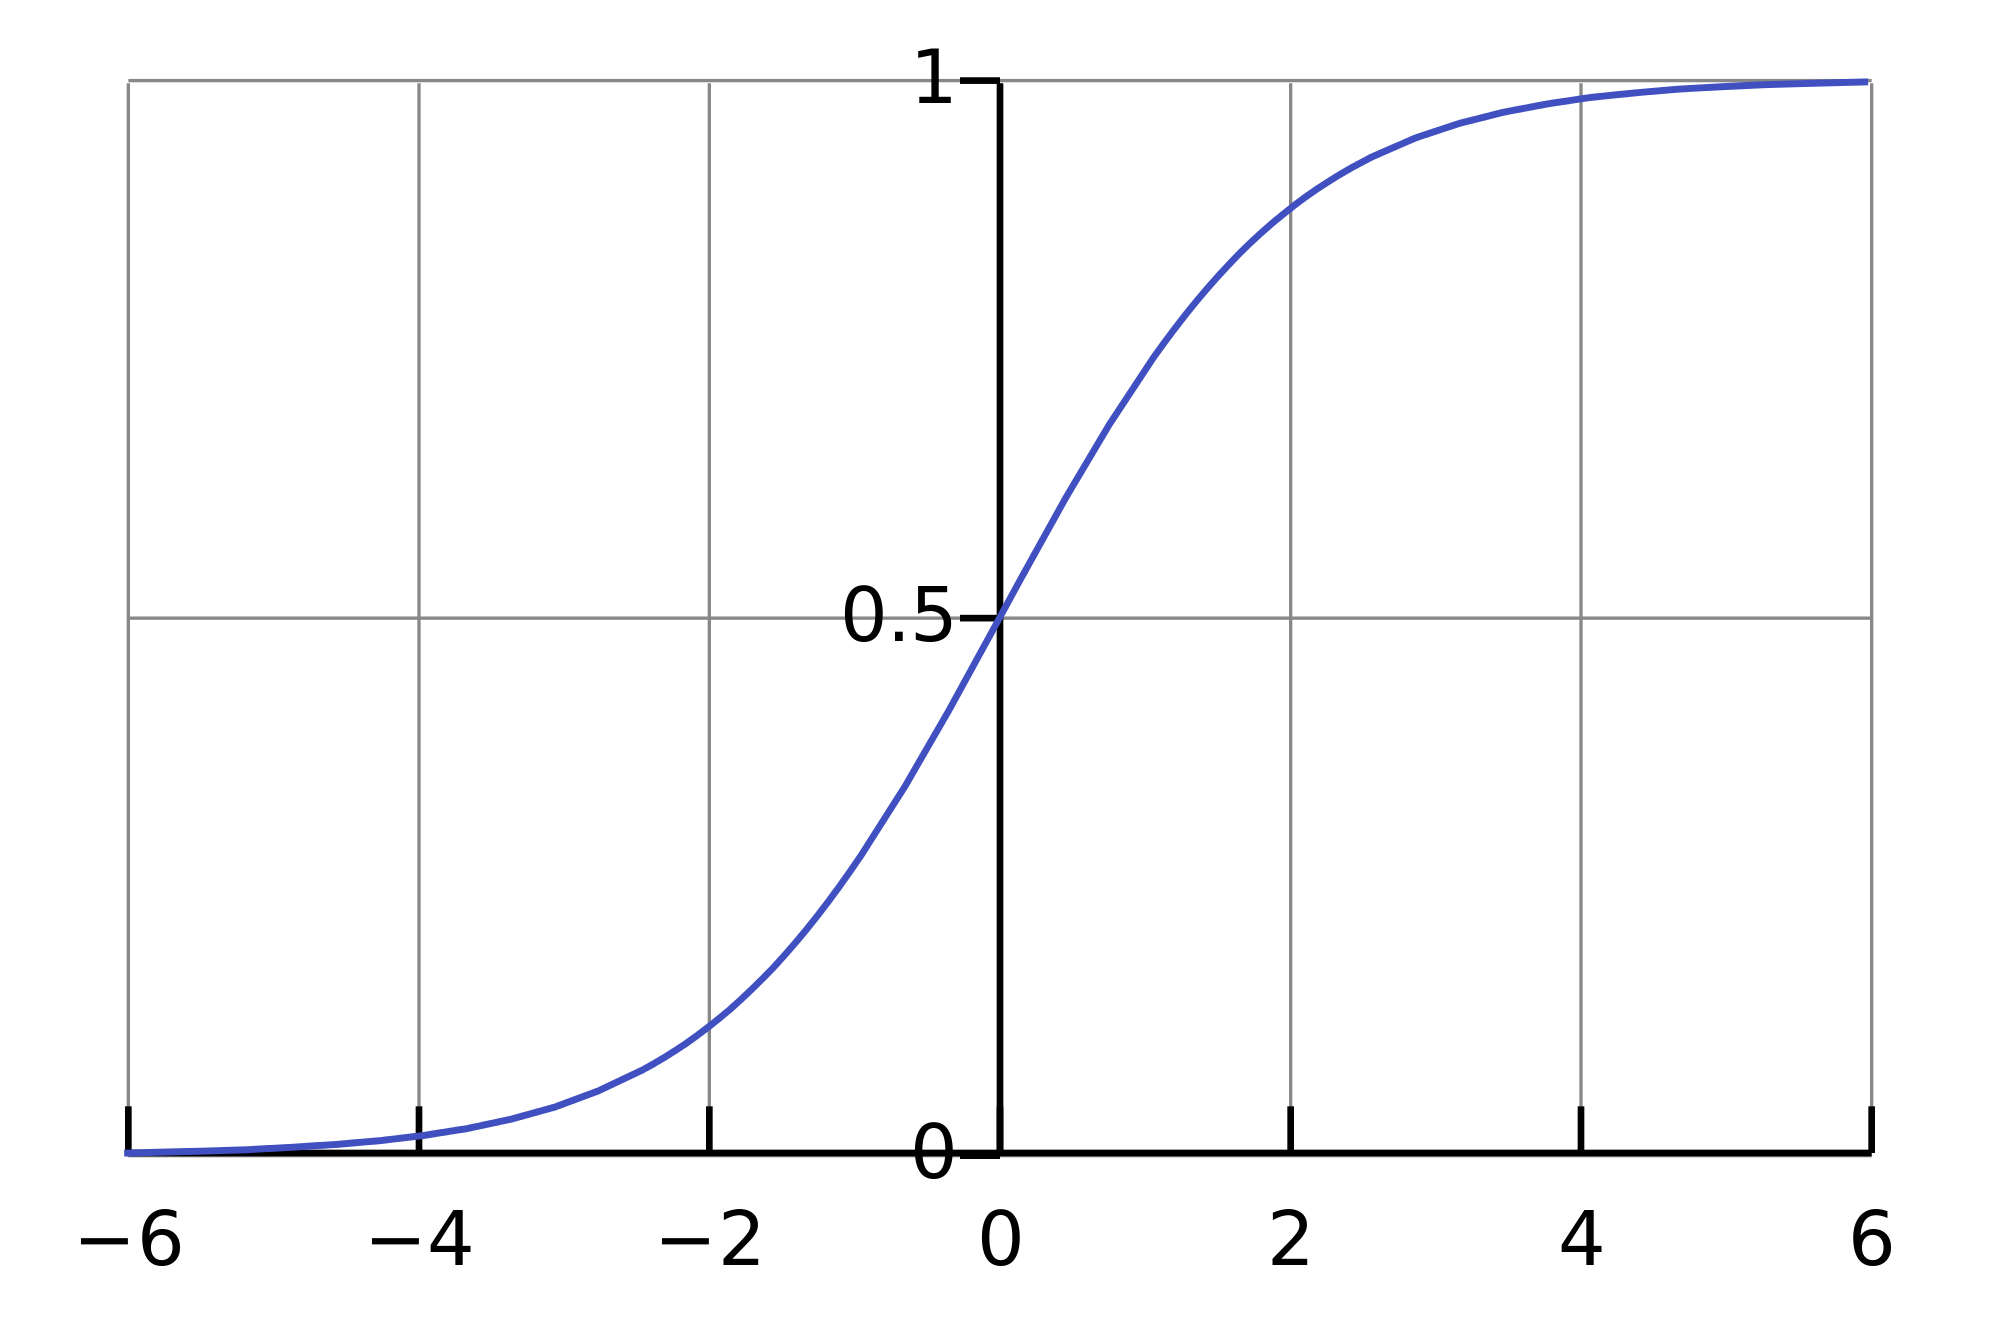
\includegraphics[width = 175px]{sig.png}
\end{frame}

\begin{frame}
\frametitle{Other Components of a Basic Neuron}
We can introduce a parameter to the sigmoid function, to control the steepness, but what if we wish to adjust where the increase begins to happen? 
\begin{block}{Bias}
The Bias is simply a constant parameter that is added to the Adder to "Bump" the input a little. I'll explain further:
\end{block}

\end{frame}

\begin{frame}
\frametitle{A diagram of a neuron}
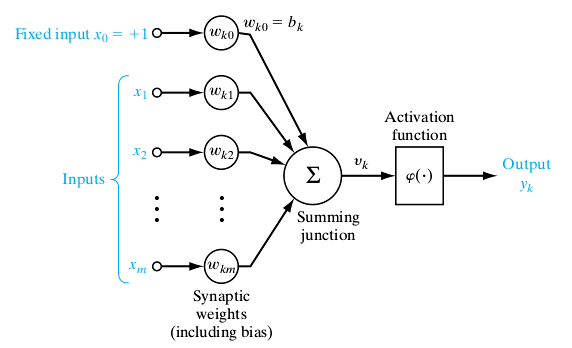
\includegraphics[width=200px]{neurond.png}


The output of a neuron can be expressed as follows:
$v_k=\Sigma_{j=1}^{m}w_{kj}x_j+b_k$ is the "Induced local field" of the neuron, where the bias "bumps" the input a little to induce the activation a little sooner or later.

$y_k = \phi(v_k)$ is then the outgoing signal from the neuron.
\end{frame}

\subsection{Single Layer Perceptron}
\begin{frame}
\frametitle{Single Layer Perceptron}
\begin{itemize}
\item We now have the terminology to examine our first Neural Network! The Single Perceptron! Yay!

\item A single layer perceptron is a binary classifier that maps an input to a binary value based on the weight that the features have. It is basically a neuron all on it's own which uses the Threshold function for activation.
\end{itemize}
\end{frame}

\begin{frame}
\frametitle{Single Layer Perceptron}
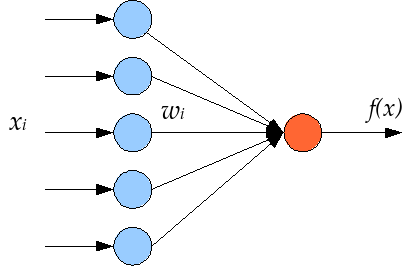
\includegraphics{slp.png}
\end{frame}

\begin{frame}
\frametitle{Single Layer Perceptron}
\begin{itemize}
\item The Single Perceptron will classify based on a positive or negative output.

\item The data in question must be linearly separable. By this we mean the existence of a hyperplane "Decision boundary" in which the two classes can be split apart.
\item This plane will simply be where $\Sigma w_ix_i + b = 0 $
\item The challenge is determining what the weights should be for the decision boundary to be correct. This is where \textbf{learning} occurs using a training set.
\end{itemize}
\end{frame}

\begin{frame}
\frametitle{Fun facts!}

\begin{itemize}
\item There is a theorem called the \textbf{Perceptron Convergence Theorem}
that proves if the training set is linearly separable, then the perceptron will converge to the correct weights that define the decision boundary.
\item The SLP is related to SVMs in that an SLP with an "Optimal Decision Boundary" combined with the Kernel Trick is the basis for SVMs.
\item There is also an equivalency between logistic regression and SLPs! 
\end{itemize}
\end{frame}

\section{Multi-Layer Perceptrons}
\subsection{Multi-Layer Perceptrons}
\begin{frame}
\frametitle{Multi-Layer Perceptron}
\begin{itemize}
\item Although the SLP can generalize to multi-class problems, we can do better.
\item The Multi-Layer Perceptron, as expected introduces more than one layer to the perceptron model (Beside the input and output layer) on which to train weights. 
\item MLPs employ a learning technique called Back Propagation.
\end{itemize} 
\end{frame}

\begin{frame}
\frametitle{Simple MLP}
\begin{itemize}
\item The most basic MLP has a single hidden layer.
\item We can view a MLP as a fully connected directed graph where each layer is connected to the next.
\item Everything except the inputs are neurons, which must have non-linear activation functions. (So that it doesn't collapse to a SLP)
\end{itemize}
\end{frame}
\begin{frame}
\frametitle{Simple MLP}

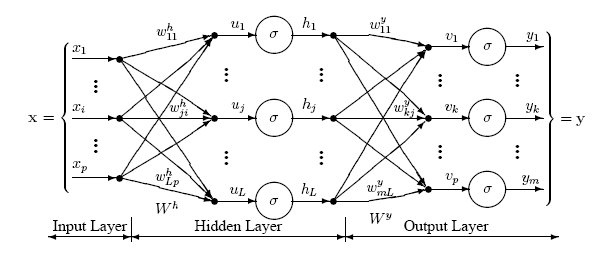
\includegraphics[width=300px]{mls.jpg}

\end{frame}

\begin{frame}	
\frametitle{So, how does it learn?}
\end{frame}
\end{document}